\documentclass[letterpaper,12pt]{article}
\usepackage[utf8]{inputenc}

\usepackage[T1]{fontenc}
\usepackage{tgtermes} %%%font

\usepackage{geometry}
\usepackage{amsmath}
\usepackage{float}
\usepackage{graphicx}
\usepackage{subcaption}
\usepackage{amssymb}
\usepackage{adjustbox}
\usepackage{wrapfig} %%imagen envuelta por un texto
\usepackage{xcolor}
\usepackage{fancyhdr}

\title {\textbf{Integrales}}
\author{Notas importantes por Deniso Xocuis}
\date{12 de agosto de 2023}
\geometry{top=2cm, bottom=2cm, left=2cm, right= 2cm} %%margen
\graphicspath{{images/}}
\parindent=0pt %%justificado

\begin{document}
\maketitle
\newpage
%%%%%%%%%%%%%%%%%%%%%%%%%%%%%%%%%%%%%%%%%%%%%%%%%%%%%%%%%%%%%%%%%%%%%%%%%%%%
\begin{sloppypar} 

\section{Definición}
Dentro del \textbf{Cálculo} encontramos las integrales mejor conocidas como "el área bajo la curva".
\vspace{0.3cm}\\
Se dice que una función es una \textbf{antiderivada o primitiva} de $f$, en un intervalo $I$ si F'(x) = f(x). Cuando se resuelve una ecuación diferencial de la forma $\frac{dy}{dx} = f(x)$ es conveniente escribirla en la forma diferencial equivalente $dy = f(x) dx$.

La operación para determinar todas las soluciones de esta ecuación se denomina antiderivación (o integración indefinida) y se denota mediante un signo integral. 
\begin{figure}[H]
    \centering
    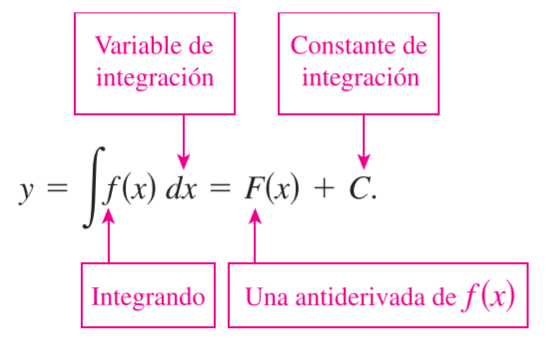
\includegraphics[width=0.4\textwidth]{intdef.png}
\end{figure}

\section{Integración indefinida}
$\displaystyle \int \frac{1}{x^3}$ dx = $\int x^{-3}$ dx = $\displaystyle \frac{x^{-3+1}}{-3+1} = \frac{x^{-2}}{-2}$ + C = $\displaystyle - \frac{1}{2x^{2}}$ + C 
\vspace{0.3cm}\\ 
$\int \sqrt{x}$ dx = $\int x^{\frac{1}{2}}$ dx = $ \displaystyle \frac{x^{\frac{1}{2} + 1}}{\frac{1}{2} + 1} = \frac{x^{\frac{3}{2}}}{\frac{3}{2}} = \frac{2x \sqrt{x}}{3}$ + C 
\vspace{0.3cm}\\
$\int 2 \sin{x}$ dx = $ 2 \int \sin{x} $ dx = $ -2 \cos{x}$ + C 
\vspace{0.3cm}\\ 
$\displaystyle \int \frac{\sin{x}}{\cos^{2}{x}}$ dx = $\displaystyle \int \frac{1}{\cos{x}} \cdot \frac{\sin{x}}{\cos{x}}$ dx = $\int \sec{x}\tan{x}$ dx = $\sec {x} $ + C
\vspace{0.3cm}\\ 
$\displaystyle \int \frac{x+1}{\sqrt{x}} $ dx = $\displaystyle \int \frac{x}{\sqrt{x}} dx + \int \frac{1}{\sqrt{x}}$ dx = $\int x \cdot x^{- \frac{1}{2}} dx + \int x^{-\frac{1}{2}} dx$ = $\displaystyle \frac{2x\sqrt{x}}{3} + 2\sqrt{x} $ = $\displaystyle 2\sqrt{x} \left(\frac{x}{3} + 1\right) = 2\sqrt{x} \left(\frac{x + 3}{3}\right) = \frac{2}{3} \sqrt{x} \left(x+3\right) + C$

\section{Método de sustitución o cambio de variable}
El papel de sustitución en la integración es comparable al de \textbf{regla de la cadena} en la derivación. La regla de la cadena establece que: 

$$\frac{d}{dx} [F(g(x))] = F'(g(x))g'(x)$$

De acuerdo con la definición de una antiderivada o primitiva, se sigue: 

$$\int F'(g(x))g'(x) dx = F(g(x)) + C$$

Y si u = g(x) entonces du = g'(x) ...\dots

$$\int f(u) du = F(u) + C$$

A tomar en cuenta:
\begin{itemize}
    \item elegir u (ecuación interior)
    \item derivar u 
    \item despejar du 
    \item reemplazar por u 
    \item integrar 
    \item reemplazar por variable original 
\end{itemize}

Consejo: la u comúnmente es la ecuación más larga 
\section{Regla general de la potencia}
$$\int u^{n} du = \displaystyle \frac{u^{n+1}}{n+1} + C, n\neq -1 $$

\section{Cambio de variable para integrales definidas}
$$\int_{0}^{1} x(x^2 + 1)^3\,dx $$

\textbf{Solución.} Para calcular esta integral, sea $u = x^2 + 1$. Después, 
$$u = x^2 + 1 \Longrightarrow du = 2x dx$$

Antes de sustituir, determinar los nuevos límites superior e inferior de integración.

\textit{Límite inferior}. Cuando x=0, u = $0^2$ + 1 = 1.

\textit{Límite superior}. Cuando x=1, u = $1^2$ + 1 = 2.

Ahora, es posible sustituir para obtener.
$$ = \frac{1}{2} \int_{1}^{2} u^3 du $$

$$ = \frac{1}{2} \cdot \left[\frac{u^4}{4}\right]_{1}^2 $$

$$ = \frac{1}{2} \left[ 4 - \frac{1}{4}\right] = \frac{15}{8}$$

\section{Integración por partes}



\end{sloppypar}
\end{document}